\documentclass[../598comp.tex]{subfiles}


\date{05-04}



\begin{document}

\section{05-04}

\subsection{Logisitics}
\begin{enumerate}
  \ii
  Potentially an oral final exam
  \ii
  Too many assignments to grade at the fast pace. Students will self grade their homeworks, and a few will be chosen at random to see if people are being honest in their self evaluation
  \ii
  All assignments are to be completed in Latex
  \ii
  Fact means he'll say it and not prove it.
\end{enumerate} 

\subsection{Schedule}
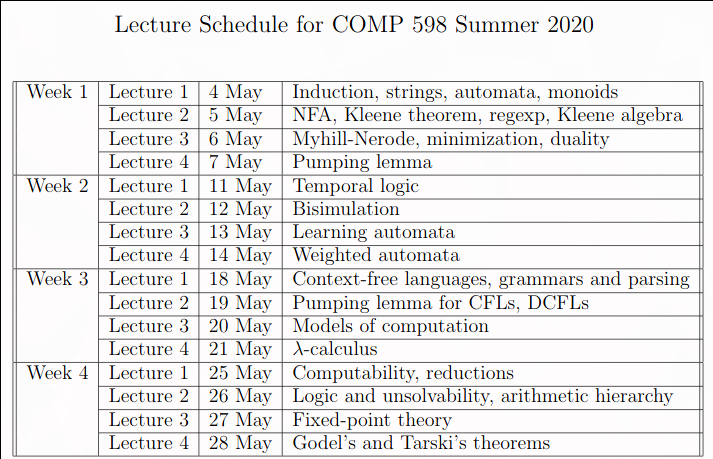
\includegraphics[width=\textwidth]{screenshot-03}

\begin{definition}[Equivalence Relation]
 An equivalence relation $R$ on a set $S$ is a set of pairs $R \subseteq S \times S$ such that (write $xRy$ for $(x, y) \in R$)
 \begin{enumerate}
  \ii$xRx$
  \ii$xRy \Rightarrow yRx$
  \ii$xRy \ \wedge \  yRz \Rightarrow xRz$
 \end{enumerate} 
\end{definition} 
\begin{definition}[Equivalence Relation]
  
$[x] \coloneqq \{y | xRy \}$ is the equivalence class of x

The set of equivalence classes forms a \ul{partition} of $S$. Prove this as an exercise.

\end{definition} 
\begin{definition}[Partial Order]
  Abstraction of comparison. Not all elements can be compared. A binary relation on a set $S$. Big difference is no symmetry.
  \begin{enumerate}
    \ii
    $x \leq x$
    \ii
    $x \leq y \wedge y \leq x \Rightarrow x = y$
    \ii
    $x \leq y \wedge y \leq z \Rightarrow x \leq z$
  \end{enumerate} 
  Example of taking subsets and ordering them by inclusion. This is a typical partial ordering that is not total. The real numbers are a total ordering.
\end{definition} 

\begin{definition}[Well-founded order]
  Given a p.o.set (partially ordered set) $(S, \leq)$ and $U \subseteq S$, we say that $u \in U$ is a \ul{minimal element} of $U$ if $\forall v < u, \ v \notin U$. There can be infinitely many minimal elements, or none. 
  \begin{example}
    \ii[]
    \ii
    Negative integers has no minimal element
    \ii
    Non negative integers in which 0 is the smallest
    \ii
    Strictly positive rational numbers has no minimal element
  \end{example} 
  A partially ordered set $(S, \leq)$ is said to be \ul{well-founded} if every non-empty subset $U$ \ul{has} (powerful word, an existential qualifier) a minimal element. 
\end{definition} 

\begin{example}
  Examples
  - Non-negative integers
    These are well founded.
  - The positive rational numbers
    These are not well founded
  - Pairs $N \times N$ where $(m, n) \leq (m', n')$ if $m < m' \vee (m = m \wedge n \leq n').$
    Between (1, 17) and (2, 5) there are infinitely many elements, but do not be fooled there is still a minimal element.
\end{example} 
 

\begin{fact}
  An order is well founded if and only if there are no infinite strictly decreasing sequences (chain) $x_1 > x_2 > x_3 > \cdots$.
  \\
  An order that is both totally ordered and well-founded is called a well order.
\end{fact} 

% Termination proofs look like this.


\begin{theorem}[Zermelo's Theorem]
  Every set can be given a well order assuming the \ul{axiom of choice}. People don't want to believe this because no one can figure out how to write a well ordering of the real numbers.
\end{theorem} 
\begin{note}
  Zermelo's well ordering principle, axiom of choice, and zorn's lemma are equivalent.
  Zorn's lemma is something people don't want to give up.
\end{note} 

\subsection{Principle of Induction}

\begin{definition}[Predicate]
  "predicate". you're in the set if you satisfy property of predicate. "predicate is a statement that may be true or false depending on the values of its variables". "The set defined by P(x) is written as {x | P(x)}, and is the set of objects for which P is true."
\end{definition} 

$(S, \leq)$ is \ul{inductive} if $\forall P, \ \forall x \in S, \ \forall y < x, P(y) \Rightarrow P(x)$

Not every order is inductive. Minimal element takes care of the base case. Which orders are inductive, and which are not?
\begin{theorem}
  An order is inductive if and only if it is well founded.
  \begin{proof}
    \begin{enumerate}
      \ii[]
      \ii
      Assume $V \coloneqq \{s \in S \ | \ \neg P(s)\}$ is not empty. Which would contradict the principle of induction. Then $\forall y < v_0, \ y \notin V$ and $P(y)$. But then this implies $P(v_0)$. So then $V = \varnothing$. i.e. $\forall x \ P(x)$.
      \ii
      Ind $\Rightarrow$ Well founded. 
      Assume $U \subseteq S$ has no minimal element. $P(x) \coloneqq x \notin U$.
      $\forall x (\forall y < x P(y)) \Rightarrow P(x)$. We know this because if all y is less than x, and $y \notin U$ by the predicate, then $x \notin U$ or else it would be a minimal element of $U$.
      \\\\
      Induction says that $\forall x P(x) \Rightarrow U = \varnothing$  and hence $(S, \leq)$ is well founded because all sets have a minimal element.
    \end{enumerate} 
  \end{proof} 
\end{theorem} 

** Emmy Noether
$\Sigma = \{a, b\}. \Sigma^* = \{\epsilon, a, b, aa, ab, \cdots\}$

Under lexicographic ordering this is \ul{not} well founded.

\subsection{Strings}
A finite set is called an alphabet. $\Sigma^*$ is a set of \ul{finite} sequences. The number of such sequences is infinite. $\epsilon$ is the symbol for the empty word. A subset of the set of sequences is called a language.

\begin{definition}[monoid]
  A \ul{moinoid} is a set $S$ with a binary operation $\cdot$ and a unit $e$. 
  \begin{enumerate}
    \ii
    $\forall x, y, z \in S, \ x \cdot (y \cdot z) = (x \dot y) \cdot z$
    \ii
    $\forall x \in S, \ x \cdot e = e \cdot x = x$
    \ii
    Monoids are not necessarily commutative. If we have that $\forall x, y, \ x \cdot y = y \cdot x$ then we get a special kind of monoid called a commutative monoid.
    \ii
    If there is an inverse operation, it is a group. Monoid's are a general form of group.
  \end{enumerate} 
\end{definition} 

\begin{example}
  \begin{enumerate}
    \ii[]
    \ii
    $\Sigma^*$ with concatenation and $\epsilon$ is a monoid, but it is not commutative. $aab \cdot ba = aabba$.
    \ii
    $\forall x, y, z$ if $xy = xz \Rightarrow y = z$ is a cancellative monoid.
  \end{enumerate} 
\end{example} 
 
\end{document}
